%% ------------------------------------------------------------------------- %%
\chapter{Test-Driven Development}
\label{cap:tdd}

Métodos ágeis de desenvolvimento de software focam sempre em constante
feedback, seja ele da equipe em relação ao cliente, ou da equipe em relação a
qualidade (interna e externa) do código produzido. Por esse motivo, muitas das
práticas sugeridas por esses métodos tentam aumentar o quantidade e a qualidade
desse feedback; a ideia da programação pareada, por exemplo, é dar retorno
sobre o código alguns segundos após ele ter sido escrito.

Test-Driven Development (TDD), popularizada pelo Kent Beck através de seu livro
\textit{TDD: By Example} em 2001 \cite{TDDByExample}, é mais uma das práticas
ágeis onde o foco é dar feedback. TDD tem grande importância durante o ciclo de
desenvolvimento já que, conforme sugerido pelas práticas ágeis, o design de um
software deve emergir a medida que o software cresce. E, para responder
rapidamente a essas alterações, é necessário um constante feedback sobre a
qualidade interna e externa do código.

A velocidade que a prática dá retorno ao desenvolvedor possibilita que o mesmo
tome decisões de design sobre o código enquanto o custo de mudança ainda é
baixo. Segundo Vanderburg, TDD dá feedback em questão de minutos, e sua
velocidade só é inferior a da programação pareada. O gráfico pode ser visto na
figura \ref{fig:agile-feedback}.

% TODO: traduzir figura do meu gdocs
\begin{figure}
  \centering
  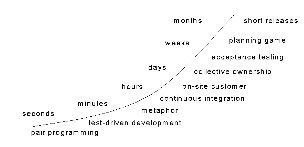
\includegraphics[scale=1]{agile-feedback}
  \caption{Práticas de XP e Tempo de Feedback}
  \label{fig:agile-feedback}
\end{figure}

Em uma definição mais formal, TDD é a arte de produzir testes automatizados para
código de produção, usando esse processo para guiar o design e a programação.
Para cada pequeno pedaço de funcionalidade, o desenvolvedor deve primeiro
escrever um teste que especifique e valide o que o código irá fazer. O
programador então produz somente o código necessário para fazer esse teste
passar. Então ele refatora (simplifica e clareia) tanto o código de produção
quanto o código de testes \cite{agilealliance-tdd} \cite{tdd-taxonomy}.

Na prática, TDD obriga que o programador escreva um código novo apenas se houver
um teste automatizado falhando, e faz com que ele remova duplicação de dados e
de código constantemente. Esse ciclo, exemplificado na figura
\ref{fig:red-green-refactor} é também conhecido como Vermelho-Verde-Refatora
(ou Red-Green-Refactor), já que lembram as cores que o programador geralmente
vê quando faz TDD: o vermelho geralmente significa que o teste está falhando, e
o verde quando o teste foi executado com sucesso.

\begin{figure}
  \centering
  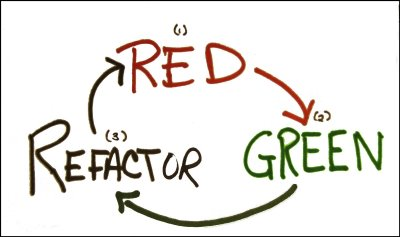
\includegraphics[scale=0.6]{ciclo-tdd}
  \caption{O ciclo Vermelho-Verde-Refatora}
  \label{fig:red-green-refactor}
\end{figure}

Apesar de ter o termo "teste" no nome, TDD não é uma prática de testes.
Um ponto interessante a ser notado é que nenhum livro sobre TDD \cite{GOOS}
\cite{TDDByExample} \cite{astels-tdd}, discute em momento algum qualquer
prática conhecida da área de testes de software, como análise do valor-limite ou
grafo de causa-efeito \cite{art-of-sw-testing}, o que leva a crer que os
benefícios de TDD não são os mesmos da área de testes.

% TODO: citar
Na opinião de muitos autores conhecidos, como Kent Beck, Martin Fowler e Robert
Martin, essa mudança na ordem do ciclo de desenvolvimento tradicional, apesar de
simples, agrega diversos outros benefícios ao código produzido: simplicidade,
foco, melhor design, entre outras.

% TODO: citar tddesign
Apesar da criação de testes ser algo intríseco ao processo, TDD é uma prática
que auxilia o desenvolvedor a desenhar classes mais flexíveis, mais coesas e
menos acopladas. Os testes são a ferramenta que o programador utiliza para
validar o design criado. Por esse motivo, muitos se referem a TDD como
\textit{Test-Driven Design}, ou seja, design guiado pelos testes.

Muitos autores afirmam que TDD é na verdade uma prática de design
\cite{tdd-taxonomy} \cite{aim-fire}, e citam sempre a famosa frase do Ward
Cunningham, um dos pioneiros da Programação Extrema: \textit{Test-First
programming is not a testing technique} que, em uma tradução livre, significa
\textit{Programação Teste Primeiro (Test-First Programming) não é uma prática
de testes}.

%% ------------------------------------------------------------------------- %%
\section{Definições incompletas}

Apesar do foco da prática em design, é possível encontrar muitas definições que
não levam isso em conta. Algumas delas levam em consideração apenas a ideia da
inversão da ordem de desenvolvimento, aonde o programador deve primeiro escrever
o teste e depois escrever o código que faça o teste passar.

Um exemplo disso é a definição que pode ser encontrada no livro \textit{JUnit
in Action} \cite{junit-in-action}: \textit{Test-Driven Development é uma
prática de programação que instrui desenvolvedores a escrever código novo
apenas se um teste automatizado estiver falhando, e a eliminar duplicação. O
objetivo de TDD é "código claro que funcione"}.

Apesar de ser correta, ela é incompleta, já que ela não captura a parte mais
interessante da prática, que é feedback no design. Interessantemente muitos
dos artigos utilizados durante a escrita dessa dissertação apresentam uma
definição parecida, e talvez por isso muitas das pesquisas em relação à prática
avaliam os efeitos de TDD sobre a qualidade externa, algo geralmente avaliado em
técnicas de testes. Esses estudos são explicados com mais detalhes no capítulo
\ref{cap:trabalhos-relacionados}.

%% ------------------------------------------------------------------------- %%
\section{O ciclo}

% TODO fazer figura do TDD
Um programador praticante de TDD escreve os testes antes do código de produção.
Beck define esse ciclo mais especificamente da seguinte maneira
\cite{TDDByExample} e reproduzido na figura XXX:

\begin{enumerate}
	\item Adicione o teste mais simples possível; 
	\item Rode todos os testes e veja o novo teste falhar; 
	\item Escreva o código mais simples que faça o teste passar; 
	\item Rode todos os testes e veja o novo teste passar; 
	\item Refatore para remover duplicação de dados e de código.
\end{enumerate}

Ao iniciar o ciclo, o programador deve escrever o próximo teste mais simples que
ela possa imaginar que falhe; em seguida, ele deve garantir que o teste que ele
escreveu realmente falha; com o teste falhando, o programador deve escrever o
código mais simples que ele possa escrever para fazer o código passar; em
seguida, ele deve checar que o teste que antes falhava, agora passa; por fim, o
programador deve refatorar todo o código duplicado que escreveu.

Perceba que simplicidade é algo intríseco ao processo; o programador deve buscar
sempre escrever o teste mais simples que falhe e escrever o código mais simples
que faça o teste passar. Por fim, a última parte do ciclo é a que se preocupa
com um código claro e flexível; nesse momento o programador deve refatorar o
código para remover toda a duplicação de dados ou de código gerada enquanto o
programador se preocupava em fazer o teste passar da maneira mais simples.

É possível ver que a prática divide o trabalho do desenvolvedor em duas partes.
A primeira se preocupa em escrever um código que funcione. Já a segunda parte
se preocupa com um código claro, expressivo e de fácil manutenção. Ron Jeffries
fez uma famosa afirmação sobre TDD que explica essa divisão: \textit{Código
claro que funciona}. Na opinião dele, o programador primeiro se preocupa com a
parte ``que funciona'', para depois deixar o ``código claro''.

%% ------------------------------------------------------------------------- %%
\section{Efeitos no design}

Na abordagem tradicional, programadores escrevem boa parte do código antes de
testarem. Ao perceberem posteriormente um problema no design, o preço para
corrigir pode ser alto demais. Uma vantagem de escrever os testes antes é
possibilitar que o desenvolvedor tome grande parte das decisões de design
enquanto o custo de mudança ainda é baixo.

O teste é o primeiro cliente da
classe que o programador ainda está por escrever e isso faz com que ele pense
melhor a respeito do comportamento que ele espera da classe. Além disso,
programadores contemplam e decidem também sobre a interface (como nomes de
classes e métodos, tipos de retorno e exceções lançadas) que a classe terá
\cite{tdd-influence}.

Além disso, ao escrever o teste antes, o programador se força a escrever um
código que seja facilmente testável. Códigos como esse possuem algumas
características interessantes, como a facilidade para invocar o comportamento
esperado, a não necessidade de pré-condições complicadas e a explicitação de
todas as dependências que a classe possui.

Gerenciamento de dependências que, conforme comentado por Robert Martin em uma
de suas palestras \cite{bobmartin-infoq}, é uma das partes mais delicadas de
todo o processo de desenvolvimento de software. Quando as dependências são mal
gerenciadas, o código torna-se difícil de manter, de evoluir e de se reutilizar.
Alterações simples demandam grandes alterações no código, já que elas se
propagam por diversas outras classes do sistema.

TDD reduz esses problemas já que, para escrever um teste de unidade para uma
determinada classe que colabora com outra, essa classe deve ter suas
dependências explícitas e deve permitir que a implementação do colaborador seja
trocada a qualquer momento. Se isso não for feito, o programador não conseguirá
testar aquela unidade de maneira isolada; ele vai sempre depender da execução da
dependência.

Uma das possíveis maneiras de explicitar as dependências, é fazer com que a
classe as receba através do seu construtor. Dessa maneira, o teste de unidade
pode passar uma implementação falsa daquela dependência que simula os
comportamentos esperados, e por fim validar o comportamento daquela classe
isolando-a completamente.

O trecho de código abaixo mostra tipicamente a diferença entre código produzido
com TDD e código produzido sem TDD:

\begin{lstlisting}[frame=trbl]
// código gerado sem TDD
public class GeradorDeNotaFiscal {
	public void geraNotaAPartirDa(Fatura fatura) {
		NotaFiscal nf = geraNota(); 
		
		Mailer sender = new Mailer("smtp");
		sender.send(new MontadorDeCorpoDoEmail().monta(nf),
		fatura.getCliente().getEmail()); }
	
	private NotaFiscal geraNota() {
		// regra de negócio que gera a nota fiscal
	}
}

// código gerado com TDD
public class GeradorDeNotaFiscal {
	private EnviadorDeNotaFiscal enviador;
	
	public GeradorDeNotaFiscal(EnviadorDeNotaFiscal enviador) {
		this.enviador = enviador;
	}
	
	public void geraNotaAPartirDa(Fatura fatura) {
		NotaFiscal nf = geraNota(); 
		
		enviador.envia(nf);
	}
	
	private NotaFiscal geraNota() {
		// regra de negócio que gera a nota fiscal
	}
}

public interface EnviadorDeNotaFiscal {
	void envia(NotaFiscal nf);
}
\end{lstlisting}

Repare que no código gerado sem TDD, a dependência para a classe \textit{Mailer}
é implícita. É impossível testar essa classe isoladamente, já que ela própria se
encarrega de instanciar e fazer uso da sua dependência. 

% TODO: referencia para os frameworks
Já no código produzido com TDD, é usual que as dependências sejam recebidas pelo
construtor. No código acima, veja que a classe \textit{GeradorDeNotaFiscal}
recebe um \textit{EnviadorDeNotaFiscal} como dependência. Veja ainda que essa
classe não recebe um \texit{Mailer}, mas sim uma interface. Dessa forma, é muito
fácil criar uma implementação falsa \textit{EnviadorDeNotaFiscal}: basta
escrever uma classe que implemente essa interface (ou ainda fazer uso de
arcabouços que facilitam esse trabalho, como o Mockito ou JMock).

Repare ainda que a classe geradora de nota fiscal recebe uma interface criada
somente para isso e não faz uso diretamente do \textit{Mailer}. Isso acontece
devido à dificuldade de se passar uma implementação falsa dessa classe; para
fazer isso, o programador precisaria escrever muito código.

Classes altamente acopladas, além de difíceis de manter, também são difíceis de
testar, já que o programador deverá fazer uso de muitos objetos dublês para
simular o comportamento esperado das dependências.

Quanto mais difícil for a escrita do teste, maior a chance da existência de
algum mau cheiro de design. Segundo Michael Feathers, existe uma sinergia muito
grande entre uma classe com alta testabilidade e um bom design: se o
programador busca por testabilidade, ele acaba criando um bom design; se o
programador busca por um bom design, ele acaba escrevendo um design mais
testável \cite{feathers-synergy}.

O teste pode dar ainda muitos outros feedbacks sobre a qualidade do design,
além do acoplamento. Uma classe que possui muita responsabilidade (ou seja, é
pouco coesa) é também difícil de testar, já que o programador gastaria muito
tempo testando todas as possíveis possibilidades. Esse tipo de classe geralmente
apresenta código complexo. Nesse caso, o programador praticante de TDD, ao
enxergar a dificuldade da escrita do teste, refatoraria a mesma, quebrando-a em
pequenas classes.

É difícil escrever aplicações complexas, sem passar por problemas de classes
altamente acopladas ou com baixa coesão. Utilizando ou não TDD, o programador
deve conhecer as boas práticas de orientação a objetos. Mas, como afirmado
anteriormente, a vantagem do programador que utiliza TDD é o tempo que ele leva
para perceber o problema.

TDD encoraja o programador a escrever componentes fracamente acoplados, de
maneira que eles possam ser testados de maneira isolada, e em um nível maior,
combinados com outros componentes.
Programar voltado para interfaces é uma prática de orientação a objetos há muito
tempo conhecida. A ideia de pensar em classes e dar mais foco à maneira com que
elas se relacionam do que com a maneira que elas implementarão determinado
algoritmo passa a ser natural. Essa discussão é o ponto forte do livro
\textit{``Growing Object-Oriented Systems, Guided By Tests''}, escrito por
Freeman e Pryce em 2009, onde ambos abordam como a prática de TDD faz com que
o programador pense mais em abstrações e relacionamento entre elas \cite{GOOS}.

O capítulo \ref{cap:design} discute boas práticas e princípios de orientação a
objetos, que foram avaliados durante a pesquisa.

%% ------------------------------------------------------------------------- %%
\section{Efeitos na corretude do código}

Uma consequência da prática de TDD é a bateria de testes de unidade gerada.
Apesar desses testes não terem sido gerados com o foco no teste do sistema, 
ela ajuda o programador a evitar erros de regressão, aonde a implementação de
uma nova funcionalidade quebra uma outra funcionalidade já existente no sistema.

Apesar disso, seu objetivo maior é dar segurança ao programador durante as
constantes refatorações de código que o programador faz e permitir com que ele
altere o design e garanta que o comportamento ainda é o mesmo. Dave Astels chama
essa bateria de testes de \textit{testes do programador} \cite{astels-tdd}, já
que ele é ferramenta de suporte ao trabalho do desenvolvedor.

Programadores ao praticar TDD não estão focados em encontrar defeitos e
acabam por não escrever testes cobrindo todos os possíveis cenários. Por esse
motivo, a prática de TDD não é substituta para todas as práticas de testes de
software vastamente discutidas na literatura. Astels os chama de \textit{testes do
cliente}, já que visam garantir o comportamento esperado do sistema do ponto de
vista do seu usuário final.

Mesmo assim, a vantagem dessa bateria de testes, apesar de incompleta, é
novamente a quantidade de feedback recebida. Por ser uma ferramenta do
desenvolvedor, essa bateria de testes é executada o tempo todo. E, por esse
motivo, ela permite ao programador encontrar erros mais rapidamente, já que a
quantidade de código escrito entre duas execuções dessa bateria é pequena, o que
facilita no processo de depuração.

O foco deste trabalho não é observar TDD sob esse ponto de vista, mas muitos
outros estudos avaliam TDD sob esse ponto de vista e podem ser encontrados na
seção \ref{cap:trabalhos-relacionados}.

%% ------------------------------------------------------------------------- %%
\section{Simplicidade}

TDD sugere que o programador dê sempre pequenos passos (conhecidos pelo termo em
inglês, \textit{baby steps}): deve-se escrever testes sempre para a menor
funcionalidade possível, escrever o código mais simples que faça o teste passar
e fazer sempre apenas uma refatoração por vez.

Uma justificativa para tal é que quanto maior o passo que o programador dá, mais
tempo ele leva para concluir esse passo e, consequentemente ele fica mais tempo
sem feedback sobre o código. Além disso, faz com que o programador não crie
soluções mais complexas do que elas precisam ser, tornando o código, à longo
prazo, o mais simples possível.

Em seu livro, Kent Beck dá exemplos de simplicidade, e na implementação de uma
operação de multiplicação dentro de uma simples classe \textit{Dinheiro},
responsável por representar uma unidade monetária, Beck escreve o seguinte
teste e implementação \cite{TDDByExample}:

\begin{lstlisting}[frame=trbl]
    public void testaMultiplicacao() {
		Dinheiro cinco = new Dinheiro(5);
		cinco.vezes(2);
		assertEquals(10, dinheiro.valor);
	}
	
	class Dinheiro {
		\textbf{public int valor = 10;}
		
		Dinheiro(int valor) {
		}
		
		void vezes(int multiplicador) {
		}
	}

\end{lstlisting}

Repare Beck fez o teste passar da maneira mais simples possível: fez o atributo
\textit{valor} receber diretamente o valor da multiplicação. E, somente com os
testes passando, Beck refatora e remove a duplicação de dados e de código
existente (o valor 10 é informação duplicada entre o teste e o código da
classe):

\begin{lstlisting}[frame=trbl]
class Dinheiro {
	public int valor;
	
	Dinheiro(int valor) {
		this.valor = valor;
	}
	
	void vezes(int multiplicador) {
		valor = valor * multiplicador;
	}
}
\end{lstlisting}

O teste ainda continua passando, provando que a refatoração foi feita com
sucesso. Pode-se observar através do exemplo acima que os passos dados foram
sempre os menores e mais simples possíveis, ou \textit{passos de bebê}, por
assim dizer. Veja que, mesmo após diversos passos de refatoração, ainda é
possível encontrar problemas de design, como o atributo \textit{valor}
declarado como público. Seriam necessários outras rodadas de refatoração para
eliminar esse problema.

Uma confusão comum de programadores que experimentam TDD pela primeira vez é a
de que fazer passos de bebê o tempo todo faz com que a produtividade diminua.
De fato, fazer passos de bebê durante todo o ciclo faz com que o tempo de
desenvolvimento aumente, já que muitos desses passos são simples demais e
poderiam ser pulados por um programador mais experiente. 

Mas TDD não força o programador a dar passos de bebê o tempo todo, mas sim
permite que o mesmo dê passos de bebê quando achar necessário
\cite{TDDByExample}: caso o programador esteja confiante sobre o trecho de
código  que está escrevendo naquele momento, ele pode dar um passo maior;  mas
caso ele não esteja tão confiante, a prática permite a ele ir mais devagar e 
dar passos de bebê, obtendo feedback mais rápido sobre o código que está
escrevendo.

O próprio Kent Beck em seu livro afirma que não faz passos tão pequenos o tempo
todo, mas se sente seguro em saber que pode dar passos pequenos quando houver
necessidade.

No exemplo acima, o método \textit{vezes} poderia ser considerado simples por
um programador experiente, que optaria por chegar à mesma solução acima de
maneira mais rápida, tomando passos maiores. Nesse momento, a experiência do
programador deve ditar o ritmo.

O conceito de simplicidade de TDD vai além da implementação de um método; a
simplicidade do design é algo também fundamental. Em modelos tradicionais de
desenvolvimento de software, diagramas de classe são criados para tentar prever
futuras alterações no software, colocando diversos pontos de flexibilização no
modelo. Muitas dessas previsões podem não se concretizar, deixando o design
desnecessariamente complexo.

Equipes ágeis optam por não fazer o chamado \textit{big design up-front (BDUF)},
e deixar que o design emerja ao longo do tempo, mantendo o código o mais claro e
simples possível, e refatorando sempre que há necessidade. Decisões de
design são tomadas com a consciência de que elas serão alteradas no futuro
\cite{is-design-dead}.

Manter o design simples não é tarefa fácil, e TDD sugere que o programador
escreva sempre o código mais simples que atenda a necessidade. Somente se a
necessidade crescer, é que o programador deverá evoluir o design. Kent Beck
comenta em seu artigo entitulado ``\textit{Aim, Fire}'', que mesmo uma decisão que
parece simples, pode ser complicada e, sem um teste para mostrar isso rapidamente, o
programador dificilmente perceberia \cite{aim-fire}. 

É interessante a afirmação de Scott Wambler sobre como o praticante de TDD lida
com a simplicidade de design. Segundo ele, TDD pode ser definido como
``\textit{TDD = Refatoração + Test-First Design}''. Segundo ele, um programador,
antes de implementar uma nova funcionalidade, deve observar se o design atual
permite que essa funcionalidade seja implementada de maneira clara. Em caso
afirmativo, o programador segue o ciclo, escrevendo um teste que falha e
fazendo-o passar. Mas, em caso negativo, o programador deve refatorar a parte do
design afetado pela nova funcionalidade, de maneira a permitir que ela seja
implementada da maneira mais fácil possível \cite{wambler-tdd}. Perceba que na
visão dele, o programador também deve sempre optar pelo design mais simples, e
somente agregar complexidade se ela for realmente necessária.

